% begin module tangent-overview
\begin{frame}
\frametitle{The Tangent Problem}
\begin{columns}[c]
\column{.35\textwidth}
\uncover<4->{%
\psset{xunit=1cm,yunit=1cm}
\begin{pspicture}(-5,-1.4)(10,1.4)
\small
%Function formula: - ((1- ((x)^{2}))^{1/2}) 
\psplot[linecolor=red, plotpoints=1000]{-1}{1}{x 2 exp -1 mul 1 add 0.5 exp -1 mul } 
%Function formula: (1- ((x)^{2}))^{1/2} 
\psplot[linecolor=red, plotpoints=1000]{-1}{1}{x 2 exp -1 mul 1 add 0.5 exp }
\psFullDot{0.4}{0.916515139}
\psline[linecolor=blue](-0.5,1.309307341)(0.4,0.916515139 )(2.5,0) %(0,0)
\rput (2, 0.4){$t$}
\end{pspicture}
}
\uncover<5->
{
\psset{xunit=1cm, yunit=1cm}
\begin{pspicture}(-5, -5)(5,5) 
\small
\psframe*[linecolor=white](-5,-5)(5,5) 
%Function formula: 1/4 ((x)^{3})+1/4 ((x)^{2})-1/2 (x) 
\psplot[linecolor=red, plotpoints=1000]{-2}{2}{x -0.5 mul x 2 exp 0.25 mul x 3 exp 0.25 mul add add }
\psFullDot{-1}{0.5}

\uncover<6->{\psline[linecolor=black] (-1.25,-0.5)(-0.75, 1.5)
\rput[l](-1, -0.4){$l$}
}

\uncover<7->{\psFullDot{1}{0}
\psline[linecolor=blue] (2, -0.25)(-2, 0.75)
\rput[b](2, -0.2){$t$}
}
\psline[linecolor=red!1](-2.1,0)(-2.11,0)
\psline[linecolor=red!1](2.1,0)(2.11,0)
\psline[linecolor=red!1](0,-2.4)(0,-2.41)
\psline[linecolor=red!1](0,2.4)(0,2.41)
\end{pspicture} 
}
%\ \uncover<4->{%
%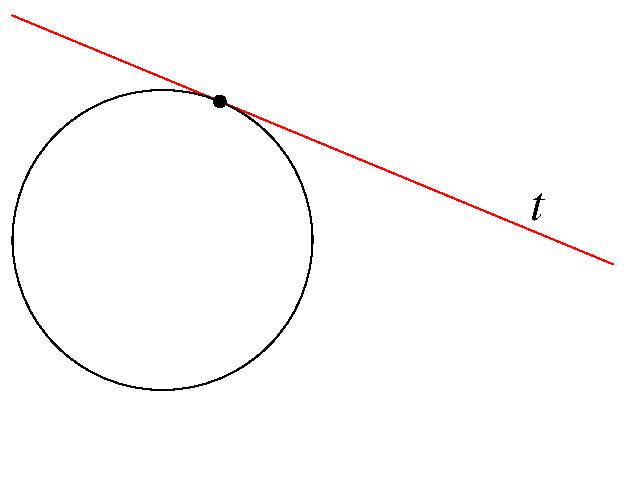
\includegraphics[height=3.5cm]{limits/pictures/02-01-tangenta.pdf}%
%}%

%\ \uncover<5->{%
%\only<handout:0| -5>{%
%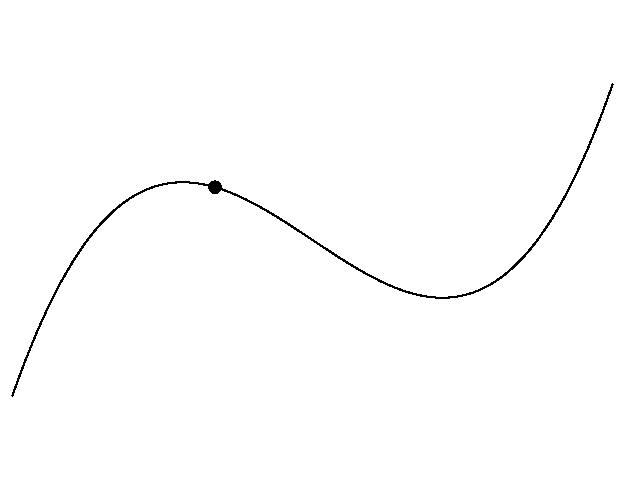
\includegraphics[height=3.5cm]{limits/pictures/02-01-tangentb.pdf}%
%}%
%\only<handout:0| 6>{%
%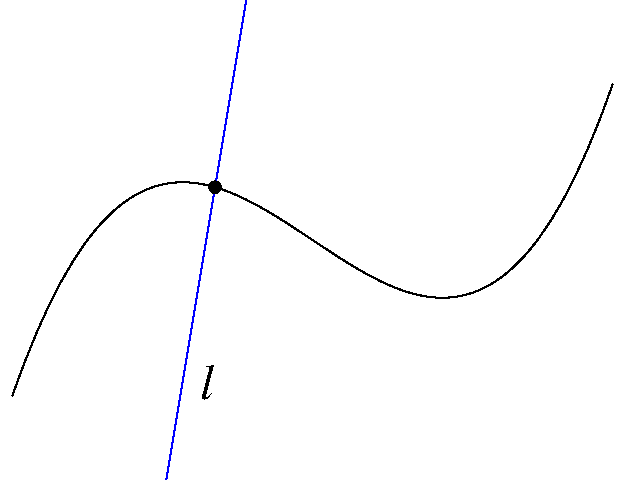
\includegraphics[height=3.5cm]{limits/pictures/02-01-tangentc.pdf}%
%}%
%\only<7->{%
%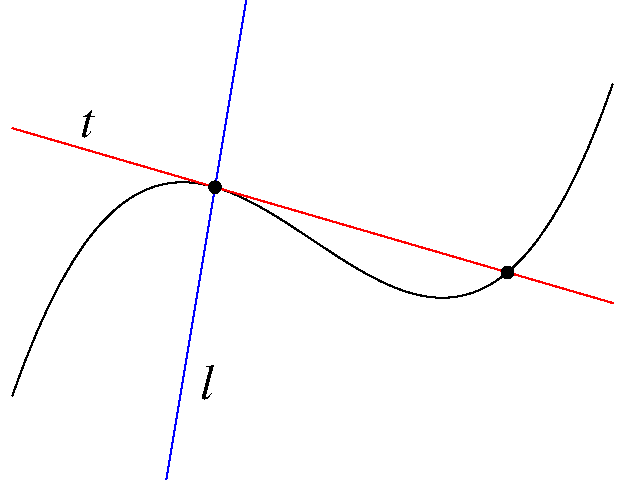
\includegraphics[height=3.5cm]{limits/pictures/02-01-tangentd.pdf}%
%}%
%}%
\column{.65\textwidth}
\begin{itemize}
\item<2->  A tangent is a line that touches a curve.
\item<3->  Moreover, a tangent should have the same ``direction'' as the curve at the point of contact.
\item<4->  For a circle, a tangent is a line that intersects the circle at exactly one point.
\item<5->  For more general curves, this definition isn't good enough.
\item<6->  The line $l$ intersects the curve at exactly one point, but it doesn't look like a tangent.
\item<7->  The line $t$ does look like a tangent, but it intersects the curve at two points.
\end{itemize}
\end{columns}
\end{frame}
% end module tangent-overview
